\section{緒言}
\label{chap:introduction}
\pagenumbering{arabic}
\subsection{研究背景}
\label{sec:back_ground}

\subsection{関連研究}
\label{sec:related_works}

\clearpage

\subsubsection{関連研究1}
\label{sec:robot_pouring_human_skill}

\subsubsection{関連研究2}
\label{sec:visual-based_pouring_motion}

\subsubsection{関連研究3}
\label{sec:tactile-based_manipulation}

\begin{figure}[h]
\centering
\subfigure[Grasping system]{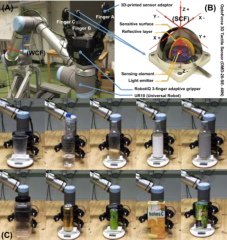
\includegraphics[width=0.35\linewidth]{images/kaboli2016tactile_pouring_overview.pdf}
 \label{fig:kaboli2016tactile_pouring_overview}}
% \subfigure[Grasping force during manipulate deformable object]{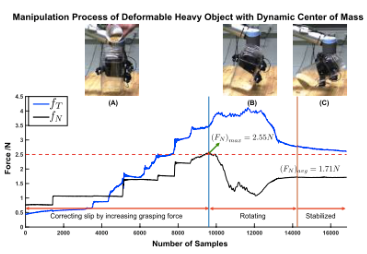
\includegraphics[width=0.35\linewidth]{images/kaboli2016tactile_sensing_force.pdf}
%  \label{fig:kaboli2016tactile_sensing_force}}
\subfigure[Deformable percentages of grasped objects]{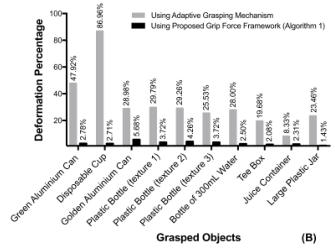
\includegraphics[width=0.5\linewidth]{images/kaboli2016tactile_grasped_object.pdf}
 \label{fig:kaboli2016tactile_grasped_object}}
\caption[Grasping system for deformable objects and result]{Grasping system for deformable objects ~\cite{kaboli2016tactile}}
\label{fig:kaboli2016tactile}
\end{figure}

\subsection{研究目的}
\label{sec:propose}

\subsection{本論文の構成}
\label{sec:organization}
本論文は全 6 章から構成される.以下に各章の概要を述べる.

\begin{itemize}
  \item \chapref{introduction}である本章は本研究の背景,関連研究と研究目的について述べた.
  \item \chapref{Consideration_pouring}では,
  \item \chapref{method}では,
  \item \chapref{experiment_pouring}では,
  \item \chapref{pouring_experiment}では
  \item \chapref{exp_robot}では,
  \item \chapref{conclusion}では本研究の結論と今後の展望について述べる.
\end{itemize}

\newpage

% This page is written in English. This page is written in English. 

\newpage